\documentclass[12pt,a4paper,oneside]{report}
\usepackage[utf8x]{inputenc}
\usepackage[english,russian]{babel}
\usepackage{cmap}
\usepackage{graphicx}
\usepackage{amsmath}
\usepackage{geometry}
\usepackage{caption}
\usepackage{titlesec}



\setlength{\jot}{2ex}

\captionsetup{labelsep=period}

\addto\captionsrussian{\renewcommand{\figurename}{Рисунок}}

\geometry{pdftex, left = 2cm, right = 2cm, top = 2.5cm, bottom = 2.5cm}

\titleformat{\chapter}
  {\normalfont\LARGE\bfseries}{\thechapter}{1em}{}
\titlespacing*{\chapter}{0pt}{3.5ex plus 1ex minus .2ex}{2.3ex plus .2ex}
\setcounter{tocdepth}{4} 

\graphicspath{ {images/} }

\begin{document}
	
\noindent \begin{minipage}{0.15\textwidth}
	
\includegraphics[width=\linewidth]{b_logo}
\end{minipage}
\noindent\begin{minipage}{0.9\textwidth}\centering
	\textbf{Министерство науки и высшего образования Российской Федерации}\\
	\textbf{Федеральное государственное бюджетное образовательное учреждение высшего образования}\\
	\textbf{«Московский государственный технический университет имени Н.Э.~Баумана}\\
	\textbf{(национальный исследовательский университет)»}\\
	\textbf{(МГТУ им. Н.Э.~Баумана)}
\end{minipage}

\noindent\rule{18cm}{3pt}
\newline
\noindent ФАКУЛЬТЕТ $\underline{\text{«Информатика и системы управления»}}$ \newline
\noindent КАФЕДРА $\underline{\text{«Программное обеспечение ЭВМ и информационные технологии»}}$\newline


\begin{center}
		\huge\textbf{ОТЧЁТ О ПРОИЗВОДСТВЕННОЙ ПРАКТИКЕ}
\end{center}



\noindent ~~Студент $\underline{\text{~~~~~~~~~~~~~~~~~~~~~~~~~~~~~~~~~~~Волков Георгий~~~~~~~~~~~~~~~~~~~~~~~~~~~~~~~~~~~~~~~~~~~~~~~}}$\newline

\noindent ~~Группа $\underline{\text{~~~~~~~~~~~~~~~~~~~~~~~~~~~~~~~~~~~~~~~~ИУ7-51Б~~~~~~~~~~~~~~~~~~~~~~~~~~~~~~~~~~~~~~~~~~~~~~~~~~~~~}}$\newline

\noindent ~~Название предприятия $\underline{\text{~~~~~~~~МГТУ им. Н. Э. Баумана, каф. ИУ7~~~~~~~~~~~~~~~~~~~~~~~~~}}$\newline



\noindent\begin{tabular}{lcc}
	Студент: ~~~~~~~~~~~~~~~~~~~~~~~~~~~~~~~~~~~~~~~~~~~~~~~~~~~~~~~~ & $\underline{\text{~~~~~~~~~~~~~~~~}}$ & $\underline{\text{~~~~Волков В.Г.~~~~~}}$     \\
	                                                                  & \footnotesize подпись, дата           & \footnotesize Фамилия, И.О.              \\
	%& &  \\
	Преподаватель:                                                    & $\underline{\text{~~~~~~~~~~~~~~~~}}$ & $\underline{\text{~~~~Волкова Л.Л.~~~}}$ \\
	                                                                  & \footnotesize подпись, дата           & \footnotesize Фамилия, И. О.             \\
\end{tabular}


\begin{center}
	\vfill
	Москва~---~\the\year
	~г.
\end{center}

\thispagestyle{empty}	
\newpage

\noindent Идивидуальное задание:\newline
Разработать программу для создания реалистических изображений с использованием алгоритма трссироваки лучей. Провести анализ cуществующих методов для построения реалистических изображений и выбрать самые подходящие.
	
	
	\tableofcontents
	\chapter*{Введение}
		\quad Компьютерная графика — область деятельности, в которой вычислительные машины 	используются с целью создания, обработки и хранения графической информации.
		
		\quad В наши дни компьютерная графика применяется во всех областях жизни человека, что вызвано широким распространением ПК, мобильных телефонов и других устройств. Особенный интерес представляют алгоритмы построения реалистичных изображений в связи с ростом производительность процессоров, памяти и графических ускорителей. Эти алгоритмы способны учитывать множество физических ,таких как отражение, преломление, прозрачность, блеск и тень. Они являются крайне требовательными к ресурсам компьютера. Их скорость работы напрямую зависит от требований к качеству и реалистичности изображения, которое должно получиться в результате работы. Трудоемкость этих алгоритмов особенно проявляется при создании динамических сцен. Необходимо найти баланс между производительностью и реалистичностью получаемого изображения.
		
		\quad Целью работы является анализ и реализация алгоритма построения реалистичного изображения с применением трассировки лучей и алгоритмов для работы с камерой наблюдателя, моделью освещения и проекцией результата на экран.
		
		\quad Для достижения поставленной цели необходимо:
		\begin{itemize}
			\item провести анализ существующих алгоритмов построения реалистических изображений, текстурирования, моделей освещений, способов представления моделей и выбрать подходящие;
    		\item реализовать выбранные алгоритмы и структуры данных;
    		\item разработать ПО позволяющее отобразить результат;
    		\item разработать интерфейс;
    		\item провести исследование реализованного алгоритма.
    	\end{itemize}
    	\quad Результатом работы будет написанное ПО для создания реалистических изображений с учётом цветов и текстур объектов и их оптических свойств, таких как отражение, преломление, прозрачность и блеск.
    \chapter{Аналитический раздел}
    	\quad В этом разделе будет представлен анализ существующих способов представления объектов, алгоритмов построения реалистического изображения, текстурирования и моделей освещения.
    \section{Описание трёхмерного объекта}
    	\quad В компьютерной графике существует множество способов представления объектов. В данной работе необходимо выделить такие способы, которые позволяет показать объём модели и наложить текстуру. В связи с этими требованиями можно рассмотреть следующие варианты:
    	\begin{itemize}
			\item геометрические примитивы;
    		\item воксельная модели;
    		\item полигональные модели.
    	\end{itemize}
    	\subsection{Геометрические примитивы}
    		\quad Примитив может быть описан некоторой функцией, принимающей параметры, например центр и радиус для сферы или ширину, высоту и глубину для параллелепипеда. В качестве таких примитивов могут выступать любые геометрические объекты: куб, конус, пирамида, сфера или цилиндр.
    		
    		\quad Достоинства:
    		\begin{itemize}
    			\item простота построения изображения модели;
    			\item малое количество информации для хранения представления. объекта.
    		\end{itemize}
    		\quad Недостатки:
    		\begin{itemize}
    			\item сложность создания реалистичной моделей из геометрических примитивов;
    			\item трудность наложения текстур.
    		\end{itemize}
    		\subsection{Воксельная модель}
    		\quad Двумерные модели можно опистать с помощью писелей. Аналогично можно и описывать трёхмерные модели из вокселей, маленьких кубиков. Они являются элементами объёмного изображения, содержащие значения элементов растра в трёхмерном виде.
    		
    		\quad Достоинства:
    		\begin{itemize}
    			\item хорошо подходит для моделирования непрерывных сред;
    			\item хорошо подходит для трассировки.
    		\end{itemize}
    		\quad Недостатки:
    		\begin{itemize}
    			\item большой расход памяти;
    			\item низкое разрешение.
    		\end{itemize}
    		\subsection{Полигональная модель}
    		\quad Полигональная модель использует полигональную сетку, которая является совокупностью связанных между собой выпуклых многоугольников (полигонов), аппроксимирующих поверхность модели. Представление модели в виде многоугольников упрощает их рендер. Чаще всего как полигон используются треугольник, так как он является простейшим многоугольником и все остальные многоугольники могут быть разбиты на треугольники.
    		
	\quad Данным способом можно описать объекты любой формы с хорошим разрешением и детализацией. Детализация зависит от количества полигонов в сетке. Время рендера напрямую зависит от количества полигонов в модели.
	
	\quad Благодаря тому что полигоны это плоские многоугольники их легко использовать для имитации неровностей, изменяя их нормали, и текстурирования, заранее указав текстурные координаты.
    		
    		\quad Достоинства:
    		\begin{itemize}
    			\item широко используются в компьютерной графике;
    			\item необходимо вычислять только координаты вершин при преобразованиях;
    			\item небольшой объём данных при хорошей аппроксимации поверхности.
    		\end{itemize}
    		\quad Недостатки:
    		\begin{itemize}
    			\item сложные алгоритмы визуализации;
    			\item аппроксимация приводит к погрешностям.
    		\end{itemize}
    		\subsection{Вывод}
    		\quad После анализа вышеописанных вариантов в качестве способа представления объектов сцены была выбрана полигональная модель. Так как в отличии от других вариантов с помощью полигональной сетки можно представить объекты любой формы в хорошем разрешении и большой детализацией, используя относительно небольшой объём памяти для хранения.
    	\section{Алгоритм построения трёхмерного изображения}
    		\quad В этом разделе будут рассмотренны алгоритмы построяния трёхмерного изображения, которые будут использоваться в написанном ПО. Эти алгоритмы являются важнейшей частью всей программы и выполняют основную работу по рендеру результирубщего изображения.
    		\subsection{Алгоритм с Z-буфером}
    			\quad Алгоритм работает в пространстве изображения и в нём используется 2 буфера: Z-буфер(буфер глубины) и буфер кадра, размер соответствуют количеству пикселей на экране. В Z-буфере находится информация о координате z для каждого пикселя, а в буфере кадра его интенсивность. В начале работы буферы заполняются минимальным значением координаты z и интенсивностью фона соответственно. Затем каждый многоугольник преобразуется в растровую форму и записывается в буфер кадра, при этом не производится никакого начального упорядочения.
    			
    			\begin{figure}[h]
					\centering
					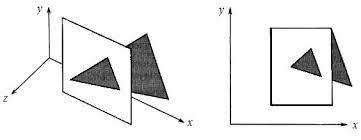
\includegraphics[scale=0.6]{zbuf}
					\caption{Пример работы алгоритма с использованием Z-буфера}
				\end{figure}
    			
				\quad В процессе работы глубина каждого нового пикселя сравнивается с глубиной, занесённой в буфер глубины. Если глубина нового пикселя меньше, то в буфер кадра заносится данные интенсивности нового пикселя, а в z-буфер новую координату z. Если же глибина нового пикселя больше, то данные в буферах не меняются.
				
				\quad Достоинствами данного алгоритма является простота его реализации и отсутствие сортировки элементов сцены. К недостаткам же можно отнести большой объём используемой памяти и трудоемкость реализации эффектов прозрачности и преломления, а также устранения ступенчатости.
			\subsection{Алгоритм с обратной трассировкой лучей}
				\quad Является модификацией простого алгоритма трассировки лучей и отличается лишь тем что лучи испускается из камеры, а не из источников света.
				
				\begin{figure}[h]
					\centering
					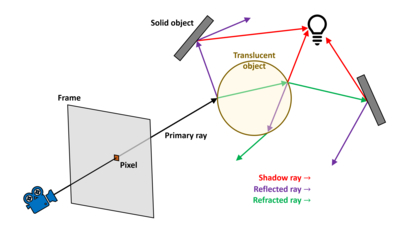
\includegraphics[scale=0.6]{trace}
					\caption{Пример работы алгоритма трассировки лучей}
				\end{figure}
				
				\quad Сам алгоритм работает по следующему принципу: из камеры выпускается луч, который называется первичным, и ищется пересечения луча с каким-либо объектом сцены. Если пересечение не находится, то результатом является фоновая интенсивнось, иначе проверяется освещенность точки пересечения первичного луча и объекта сценаа всеми источниками света. Для это пускается теневой луч в направлении каждого источника света. Если он пересекает какой-либо объект, то источник света не видим из точки пересечения, то есть объект находится в тени относительного этого источника и соответственно он не освещает данную точку. Если же теневой луч не встретил никаких объектов на своём пути, то интенсивность рассчитывается в соответствии с моделью освещения. Результатом являет суммарная интенсивность от всех видимых источников света.
				
				\quad Если тела обладает отражающими свойства, то просчитывается и испускается отражённый луч, для которого рекурсивно выполняются те же операции как и для первично. Аналогично программа работает с преломлёнными лучами.
				
				\quad Достоинства данного алгоритма является высокий реализм получаемого изображения, учёт таких физических явлений как тень, преломление, отражение. Также алгоритм легко поддаётся распараллеливанию.
				
				\quad Основным недостатком является производительность. Каждый раз необходимо просчитывать множество новых лучей, что создаёт немалую нагрузку на вычислительные устройства.
			\subsection{Вывод}
				\quad Для создания реалистичного изображения лучше всего подходит алгоритм трассировки лучей, так как он даёт наиболее приближенный к реальности результат и учитывает отражения, прозрачность и тени. Основным недостатком является его производительность. Алгоритм с использованием Z-буфера же можно использовать для предпросмотра сцены где может потребоваться рендер в реальном времени, которые трудно реализуем алгоритмом трассировкой лучей без соответствующего графического ускорителя.
		\section{Алгоритмы наложения текстур на трёхмерные объекты}
			\subsection{Афинное текстурирование}
				\quad Самый дешевый способ интерполяции между тремя текстурными координатами треугольника — использовать линейную интерполяцию с барицентрическими координатами. Введём координаты текстуры $u$, $v$. Они указвают на определённый пиксель текстуры, тексель. Для вершит полиговон изначльно заданы текстурные координаты, указываю на соответствующий тексель. Чтоб не высчитывать значения $u$ и $v$ для каждого пикселя проекции полигона, можно вопользоваться билинейной интерполяцией, используя уже известные координаты тексилей вершин треугольника. Основным недостатком этого метода является игнорирование координаты $z$, из-за чего текстура может искажатся и выглядить нереалистично.
			\subsection{Перспективно-корректное текстурирование}
				\quad Искажения в афинном текстурировании вызваны допущем что $u$, $v$ изменяются по экрану линейно. Это не так. Точные значения координат тексилей можно считать по точечным формулам, но это не эффективно. Проще воспользоваться фактом что $u/z$ и $v/z$ линейно зависят от координат проекции треугольника. Достаточно посчитать для каждой вершины $1/z$, $u/z$ и $v/z$, а затем их линейно интерполировать по асему полигону. Сами же точные значения $u$ и $v$ считаюся как: \[ u=(u/z)/(1/z) \] \[ v=(v/z)/(1/z) \]
			\subsection{Вывод}
				\quad Наиболее реалистичным методом является перспективно-корректное текстурирование, так как в его основе лежит точное тексутрирование, учитывающее перспективу в отличии от афинного метода.
		\section{Модель освещения трёхмерных объектов}
			\subsection{Модель Ламберта}
				\quad Простейшая модель освещения, чисто диффузное освещение. Считается, что свет падающий в точку, одинакового рассеивается по всем направлением полупространства. Таким образом, освещенность в точке определяется только плотностью света в точке поверхности, а она линейно зависит от косинуса угла падения. Считается по формуле:
				\[
					I = k_{d}(\vec{n}, \vec{l}),
				\]
				\quad где
				\begin{itemize}
					\item $k_{d}$ - коэффицент диффузного отражения;
					\item $\vec{n}$ -  нормаль;
					\item $\vec{l}$ - еденичные вектор, напрвленный к источнику света.
				\end{itemize}
			\subsection{Модель Фонга}
				\quad Модель расчёта освещения трёхмерных объектов, в том числе полигональных моделей и примитивов, а также метод интерполяции освещения по всему объекту. Это локальная модель освещения, то есть она учитывает только свойства заданной точки и источников освещения, игнорируя эффекты рассеивания, линзирования, отражения от соседних тел. Эта модель состоит из диффузной составляющей и зеркальной. Благодаря зеркальной составляющей на объектах появляеюся блики. Интенсивность в точке зависит от того насколько близки отражённый вектор к вектору направленному из точки падения в сторону наблюдетеля. В модели учитывается интенсивность фонового, диффузного и зеркально освещёния. Для расчёта диффузной составляющей используется модель Ламберта. Считается по формуле:
				\[
					I = k_{a}I_{a} + k_{d}(\vec{n}, \vec{l}) + k_{s}(\vec{n}, \vec{r})^n,
				\]
				\quad где
				\begin{itemize}
					\item $k_{d}$ - коэффицент диффузного отражения;
					\item $k_{s}$ - коэффицент зеракльного отражения;
					\item $k_{a}$ - коэффицент рассеянного отражения;
					\item $I_{s}$ - интенсивность фонового освещения;
					\item $\vec{n}$ -  нормаль;
					\item $\vec{l}$ - еденичные вектор, напрвленный к источнику света;
					\item $\vec{l}$ - еденичные вектор, напрвленный к наблюдателю;
					\item $n$ - степень, аппроксимирующая пространственное распределение зеркально отраженного света.
				\end{itemize}
			\subsection{Модель Уиттеда}
				\quad Модель освещенности Уиттеда является одной из самых распространенных и наиболее часто используемой моделью в методе трассировки лучей. Ипользует для расчёта интенсивности глобальноую модель освещения, учитывающую свет провзаимодействовавший с други объектами. Помимо учёта фоновой, диффузной и зеркальной компонент в этой модели ещё учитывается интернсивность отражённого и преломлённого света от других тел.
			\subsection{Вывод}
				\quad Для получения наиболее реалистических изображений была выбрана модель Уиттеда как самая подходящая и реалистичная, так как она учитывает такие эффекты, как отражение, прозрачность, преломление, тень.
	\chapter{Конструкторский раздел}
		\section{Реализация алгоритма обратной трассировки лучей}
			\subsection{Алгоритм обратной трассировки лучей}
				\quad Алгоритм обратной трассировки лучей работает следующим образом: из камеры пускается луч черерез каждый пиксель эрана и ищется его пересечения с объетами сцены. Луч выпущенный из камеры называется первичным. Пусть точка пересечения называется П1.
				
				\begin{figure}[h]
					\centering
					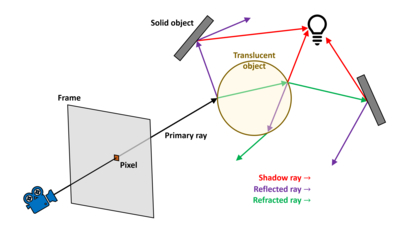
\includegraphics[scale=0.6]{trace}
					\caption{Схема работы алгоритма трассировки лучей}
					\label{fig:trace}
				\end{figure}				
				
				\quad Далее для кажого источника света определяется, видна ли для него точка П1. Для это испускается теневой луч(красная стрелка на рисунке \ref{fig:trace}) из П1. Если он пересекается с какими-либо объектами, находящимися между П1 и источником света, то точка находится в тени от это источника и не освещается им. Далее освещени считается по некой модели. Результатом будет сумма интенсивностей всех видимых источников света для П1. Если материал имеет отражающие свойства то просчитывается и испускается отражённый луч света(фиолетовая стрелка на рисунке \ref{fig:trace}) и точно так же рекурсивно обрабатывается. Аналогично происходит с преломлёнными лучами(зелёная стрелка на рисунке \ref{fig:trace}), если материал имеет преломляющие свойства.
				
				\begin{figure}
					\centering
					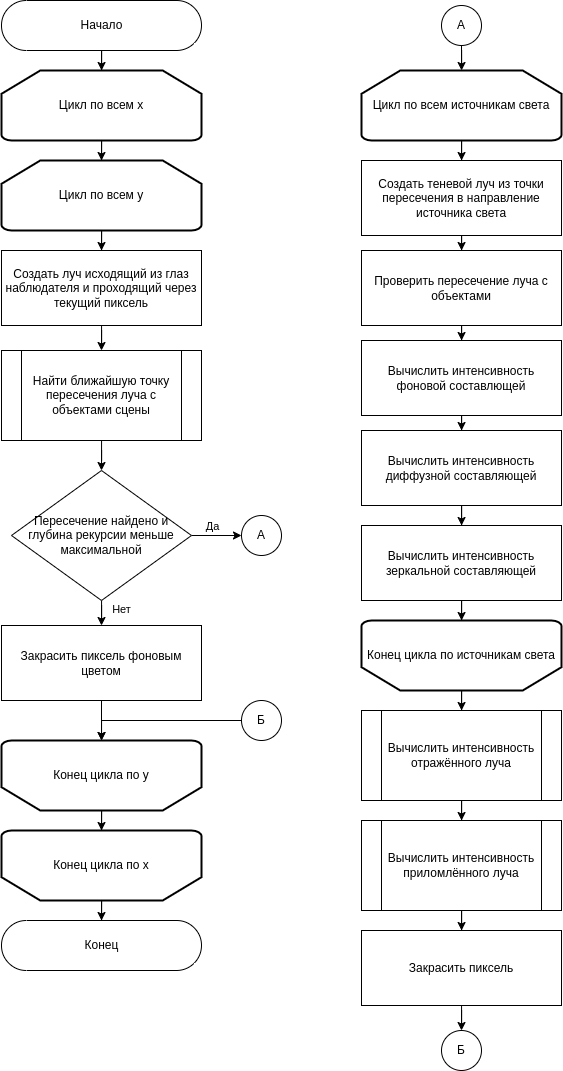
\includegraphics[scale=0.6]{trace_block}
					\caption{Блок-схема алгоритма трассировки лучей}
				\end{figure}
				
			\subsection{Нахождение пересечеия с полигоном}
				\quad Самым известным тестом на пресечение луча и треугольника является бариоцентрический тест.
				
				\begin{figure}[h]
					\centering
					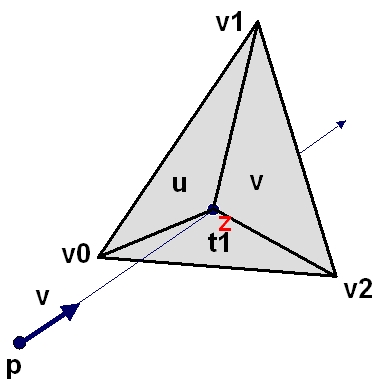
\includegraphics{intersec}
					\caption{Схема для поиска пересечения луча и треугольника}
					\label{fig:intersec}
				\end{figure}
				
				\quad Введём следующие обозначения как на рисунке \ref{fig:intersec}
				\begin{itemize}
				    \item $Z$ - точка пересечения;
    				\item $P$ - начало луча;
    				\item $t$ - расстояние от $p$ до $z$;
    				\item $\vec{d}$ - направление луча;
    				\item $V_{0}$, $V_{1}$, $V_{2}$ - вершины треугольника;
    				\item $u$, $v$, $t1$ - барицентрические координаты.
    			\end{itemize}
    			\quad Барицентрические координаты представляют собой отношения площадей маленьких треугольников к большому треугольнику. Имея 3 точки на плоскости, можно выразить любую другую точку через ее барицентричечкие координаты. 
    			\begin{equation}
					Z(u, v) = (1 - u - v)*V_{1} + u*V_{2} + v*V_{0}
					\label{eq:1}
				\end{equation}
    			\quad Уравнение (\ref{eq:1}) берется просто из определения барицентрических координат, выражая точку пересечения z.
    			\begin{equation}
					Z(t) = P + t*\vec{d}
					\label{eq:2}
				\end{equation}
    			\quad Уравнение (\ref{eq:2}) это параметрическое уравнение прямой.
    			\begin{equation}
					P + t*\vec{d} = (1 - u - v)*V_{1} + u*V_{2} + v*V_{0}
					\label{eq:3}
				\end{equation}
    			\quad Прировняв правые части уравнений (\ref{eq:2}) и (\ref{eq:3}) получаем третье уравнение, которое, по сути, является системой из 3-х уравнений с 3-мя неизвестными ($u$ ,$v$, $t$).
    			
    			\quad Проведя алгебраические преобразования получим
    			\[
    				\begin{bmatrix}
						t\\
						u\\
						v
					\end{bmatrix}
					= \frac{1}{(\vec{V}, \vec{E_{1}})}*
					\begin{bmatrix}
						(\vec{Q}, \vec{E_{2}})\\
						(\vec{V}, \vec{T})\\
						(\vec{Q}, \vec{d})
					\end{bmatrix}
				\]
				\quad где $\vec{E_{1}} = V_{1} - V_{0}, \vec{E_{2}} = V_{2} - V_{0}, \vec{T} = P - V_{0}, \vec{V} = (\vec{d} \times \vec{E_{2}}), \vec{Q} = (\vec{T} \times \vec{E_{1}})$.
			\subsection{Нахождение пересечеия с объемлющей оболочкой}
				\quad При трассировке лучей крайне неэффективно искать пересечения с каждым полигоном объекта. Лучше поместить объект в объемлюющкю оболочку и сначала проверять пересение с ней. Если луч не пересекает оболочку, то и не перескает объект сцены, находящийся в оболочке. В качестве такой оболочки будет использоваться сфера в связи спростотой поиска пересечения луча и сферы.	
				
				\quad Из уравнение луча имеем $X = A + t\vec{d}$. Уравнение для точки на поверхности серы выгядит слудуюзим образом $|X - C|^2 = r^2$. Подставив $X$ во второе уравнение получаем: 
				\[
    				|A + t\vec{d} - C|^2 = r^2
				\]
				
				\quad Обозначим $\vec{s} = A - C$, тогда
				
				\[
    				|s + t\vec{d}|^2 = (\vec{s}, \vec{s}) + 2t*(\vec{s}, \vec{d}) + t^2*(\vec{d}, \vec{d}) = r^2
				\]
				
				\quad Получилось квадратное уравнение относительно t. Дискриминант считается считается следующим образом:
				
				\[
    				D = 4*((\vec{s}, \vec{d})^2 - d^2*(s^2 - r^2))    				
				\]
				
				%\begin{equation}				
    				%t_{1,2} = \frac{-(s, d) +- \sqrt{(s, d)^2 - d^2*(s^2 - r^2)}}{d^2}
					%5\label{eq:8}
				%\end{equation}
				
				\quad Если D < 0 то объект, находящийся в объемлющей сфере, сразу можно выбрсывать из рассмотрения, так как луч его точно не пересекает.
				
				\begin{figure}[htp]
					\centering
					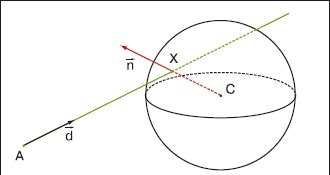
\includegraphics{sphere}
					\caption{Пересечение сферы лучём}
					\label{fig:sphere}
				\end{figure}
				
			\subsection{Ускорение алгоритма трассировки лучей}
				\quad Распараллеливания алгоритмов часто используют для ускорения работы. Алгоритм трассировки лучей отлично поддаётся распраллеливанию посколько каждый пиксель экрана обрабатыевается независимо. Можно разбить экран на сектора в виде прямоугольников, которые будут обрабатываться параллельно, независимо друг от  друга. 
				
				\quad Также можно строить иерахическую структуру оболочек, что позволит отбрасывать сразу целые группы объектов, которе не пересекает данный луч.
		\section{Реализация модели освещения Уиттеда}
			\subsection{Нахождение отражённого луча}
				\quad Для нахождения направление отражённого луча $\vec{R}$ необходимо знать только направления нормали $\vec{N}$ и падающего луча $\vec{L}$.
				
				\begin{figure}[htp]
					\centering
					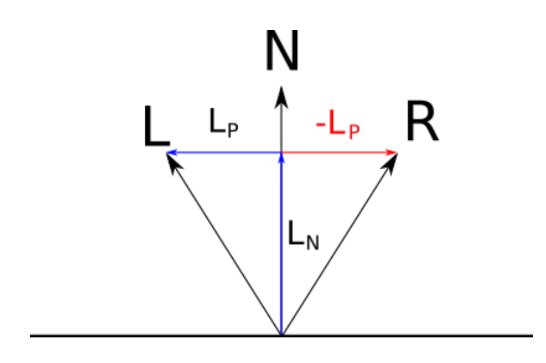
\includegraphics[scale=0.5]{reflect}
					\caption{Разложение падающего луча}
					\label{fig:reflect}
				\end{figure}
				
				\quad Падающий вектор $\vec{L}$ можно разложить на два проекции $\vec{L_{N}}$ и $\vec{L_{P}}$. Тогда $\vec{L} = \vec{L_{N}} + \vec{L_{P}}$. Так как $\vec{N}$ единичный вектор, то длинна прекции будет равна $(\vec{L}, \vec{N})$ и $\vec{L_{N}} = (\vec{L}, \vec{N})\vec{N}$. Следовательно $\vec{L_{P}} = \vec{L} - \vec{L_{N}}$. Отражённый же луч можно выразить как $\vec{R} = \vec{L_{N}} - \vec{L_{P}}$. Всё подставивив и упростив окончательно получаем $\vec{R} = 2(\vec{L}, \vec{N})\vec{N} - \vec{L}$.
			\subsection{Нахождение преломлённого луча}
				\quad Преломлённый луч $\vec{P}$ можно найти изходя их того факта что падающий и преломлённый лучи лежат в одной плоскости и из закона Снелиуса, который записывается так:
				
				\[
    				sin(\alpha)*n_{1} = sin(\gamma)*n_{2}
					\label{eq:9}
				\] 
				
				\begin{figure}[htp]
					\centering
					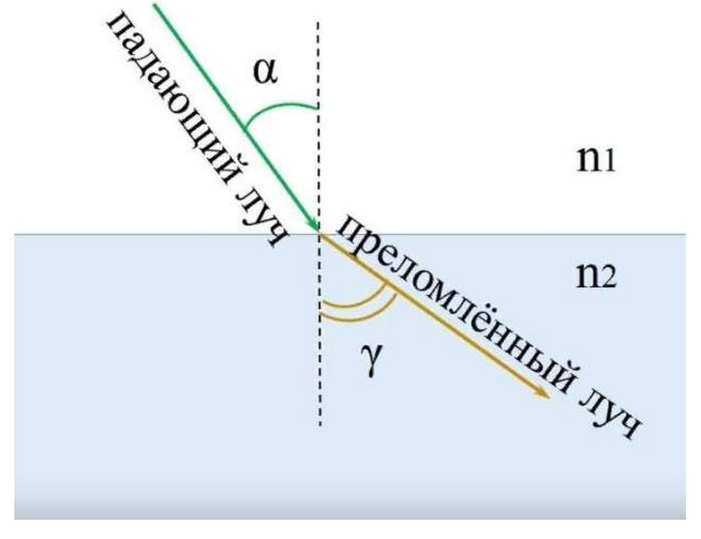
\includegraphics[scale=0.2]{refract}
					\caption{Преломление}
					\label{fig:refract}
				\end{figure}
				
				\quad Введём дополнительные обозначение $n = \frac{n_{1}}{n_{2}}$, $\vec{L}$ - падающий луч, $\vec{N}$ - нормаль. Можем получить уравнение для вектора преломлённого луча:
				
				\[
    				\vec{P} = n*(\vec{L} + cos(\alpha)*\vec{N}) - \vec{N}\sqrt{1 - sin^2(\gamma)}
				\]
				
				\quad Если подкоренное выражение отрицательно, то этот случай соответствует полному отражению.	
			\subsection{Общая реализация модели освещения Уиттеда}
				\quad Модель Уиттеда учитывает фоновое, диффузное и зеркальное освещение, а также эффеты отражения и преломления. Согласно этой модели суммарная интенсивность определяется следующим уравнением:
				\[
    				I = k_{a}I_{a}C + k_{d}I_{d}C + k_{s}I_{s} + k_{r}I_{r} + k_{t}I_{t},
				\]
				\quad где 
				\begin{itemize}
    				\item $k_{a}$ - коэффициент рассеянного отражения;
    				\item $k_{d}$ - коэффициент диффузного отражения;
    				\item $k_{s}$ - коэффициент зеокального отражения;
    				\item $k_{r}$ - коэффициент отражения;
    				\item $k_{t}$ - коэффициент преломления;
    				\item $I_{a}$ - интенсивность фонового компоненты;
    				\item $I_{d}$ - интенсивность диффузной компонеты;
    				\item $I_{s}$ - интенсивность зеркального компоненты;
    				\item $I_{r}$ - интенсивность отражённого луча;
    				\item $I_{t}$ - интенсивность преломлённого луча;
    				\item $C$ - цвет.
    			\end{itemize}
    		\subsection{Расчёт интенсивностей}
    		\quad Интенсивность диффузного отражения не зависит от положения наблюдателья. Её интенсивность в точке можно вычислить по следующей формуле:
    		\[
    			I_{d} = k_{d} * \sum I_{i}*(\vec{N}, \vec{L_{i}}),
    		\]
    		\quad где 
				\begin{itemize}
    				\item $k_{d}$ - коэффициент диффузного отражения;
    				\item $I_{i}$ - интенсивность в точке, от i-го источника света;
    				\item $\vec{N}$ - нормаль;
    				\item $\vec{L_{i}}$ - единичный вектор, направленный в строну i-го источника света.
    			\end{itemize}
    			\quad Интенсивность же зеркального отражения зависит от положения наблюдателья и её интенсивность в точке можно вычислить по следующей формуле:
    		\[
    			I_{d} = k_{s} * \sum I_{i}*(\vec{S}, \vec{R_{i}})^n,
    		\]
    		\quad где 
				\begin{itemize}
    				\item $k_{s}$ - коэффициент зеркального отражения;
    				\item $I_{i}$ - интенсивность в точке, от i-го источника света;
    				\item $\vec{S}$ - единичный вектор, направленный в строну наблюдателя;
    				\item $\vec{R_{i}}$ - единичный вектор, задающий направленние отражённого луча от i-го источника света;
    				\item $n$ - степень, аппроксимирующая пространственное распределение зеркально отраженного света.
    			\end{itemize}
    		 \quad В итоге получается следующая формула:
    		\[
    				I = k_{a} \sum I_{ai} + k_{d} * \sum I_{i}*(\vec{N}, \vec{L_{i}}) + k_{s} * \sum I_{i}*(\vec{S}, \vec{R_{i}})^n + k_{r}I_{r} + k_{t}I_{t},
			\]
		\section{Выбор используемых типов данных}
			\quad В программе будут реализованны и использованны следующие структуры данных:
			\begin{itemize}
    				\item Point3D - точка;
    				\item Vector3D - ветор;
    				\item Color - цвет;
    				\item Polygon - полигон. Хранит индексы вершин, координат нормали и  текстурных координат;
    				\item SceneObject - объект сцены. Хранит координаты вершин, нормали, текстурные координаты и полигоны;
    				\item LightObject - источник света. Хранит координаты источника света;
    				\item Camera - камера. Хранит координаты, направление и вектор указывающий наверх;
    				\item Scene - сцена. Хранит все объекты.
    			\end{itemize}
    \chapter{Заключение}
    \quad Во время выполнения поставленной задачи были рассмотренны способы представления трёхмерных объектов, алгоритмы построения реалитического изображения, методы наложения текстур и модели освещения. Были проанализированны их достоинства и недостатки и выбраты самые подходящие для реализации поставленной задачи.
    
    \quad В ходе выполенения поставленной задачи мной были изучены возмоности QT Framework, полученны знания в такой перспективной сфере компьюторной графики, как трассировка лучей с глобальным освещением.
    \chapter{Источники}
    	\begin{itemize}
    		\item Роджерс
    		\item Ray tracing in one week
    		\item Джеймс Д. Фоули, Андрис Ван Дам, Стивен К. Фейнер и Джон Ф.
Хьюз, Принципы и практика компьютерной графики, второе издание.
			\item Компьютерная графика. Рейтрейсинг и растеризация
    	\end{itemize}
\end{document}
